\documentclass{article}

\usepackage{fullpage}
\usepackage{amsmath}
\usepackage{bm}
\usepackage{esdiff}
\usepackage{cite}
\usepackage{hyperref}
\usepackage{graphicx}

\renewcommand{\vec}[1]{\bm{\mathrm{#1}}}

\graphicspath{{./res/}}

\title{Kelvin-Helmoltz Instability}
\author{Jonathan Elsner}
\date{December 11\textsuperscript{th}, 2024}

\begin{document}

\maketitle

\section{Abstract}

% Maybe look at MIT guide to abstract writing?
Kelvin-Helmholtz (KH) instability is a process that occurs at the interface
between two fluids of two differing densities, creating vortex waves. KH
Instability is a commonly occurring process in nature: it is one of the driving
forces of mixing in the ocean \cite{woods-1968}, causes clear-air turbulence on
flights and can sometimes be seen in cloud formations \cite{ludlam-1967}. It is
also thought to be a factor in heating the corona of the Sun
\cite{nasa-solar-surfer}.

\begin{figure}[h]
    \centering
    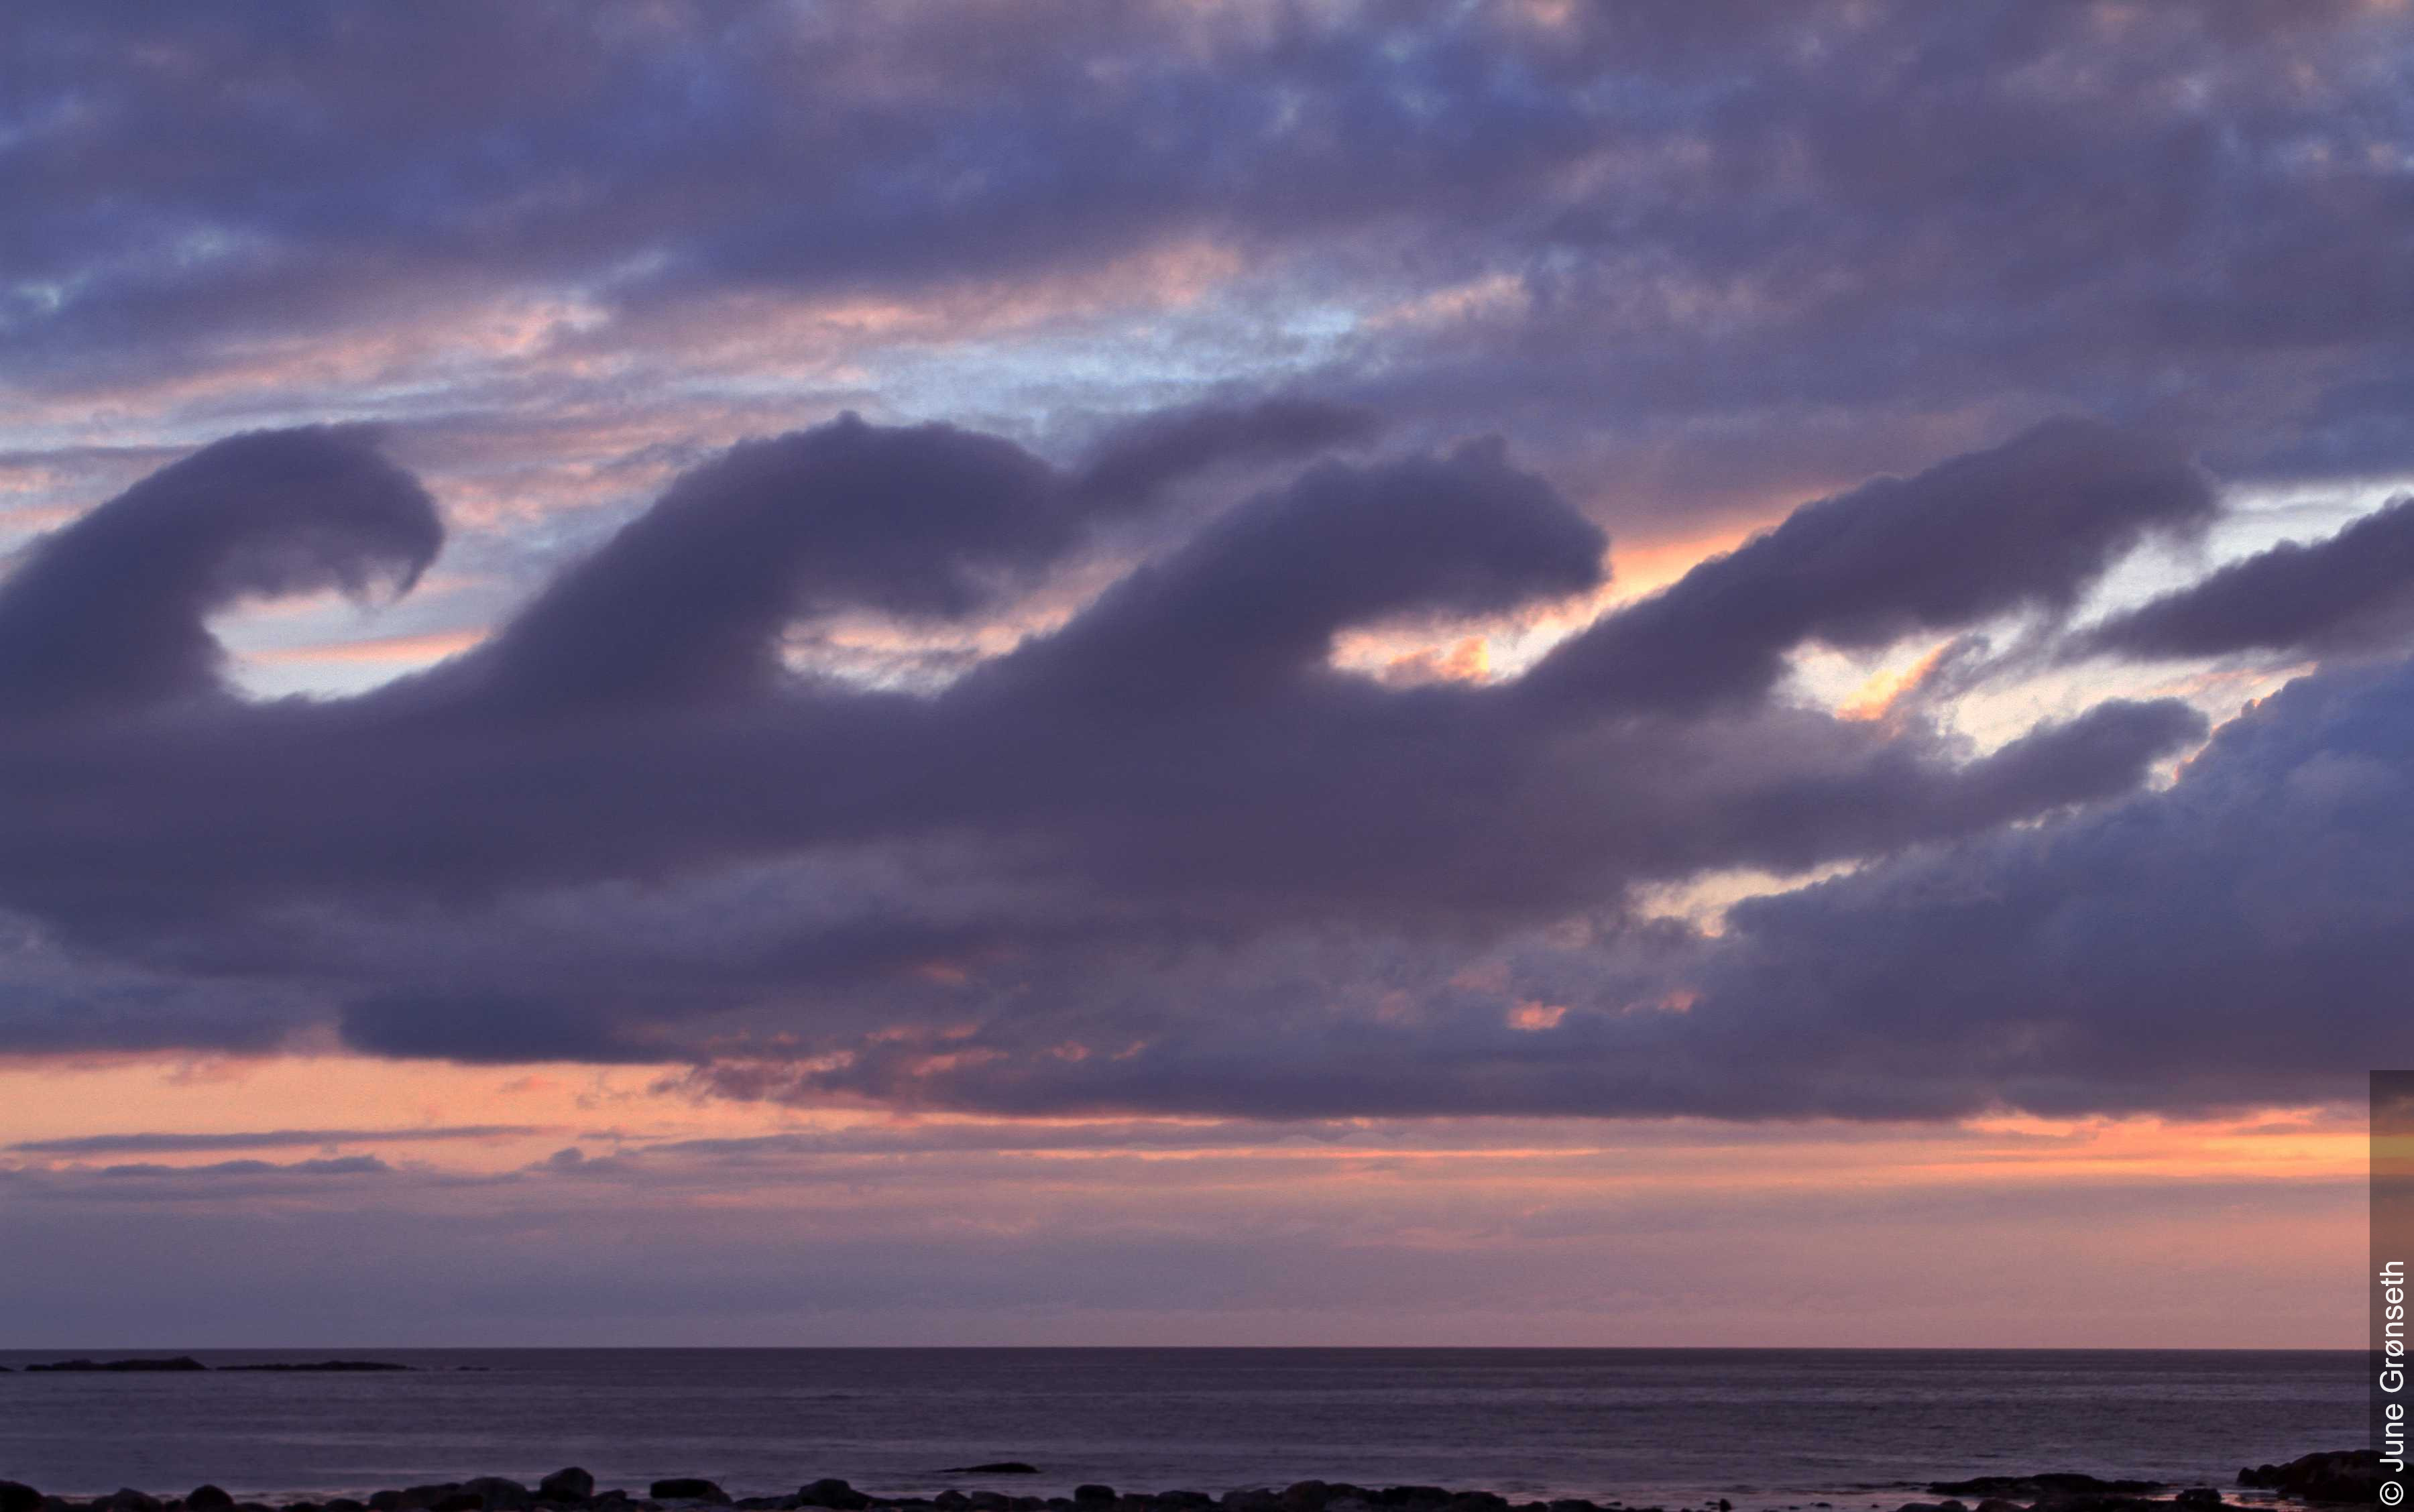
\includegraphics[width=4in]{kh-instability-clouds-2.jpg}
    \caption{Rare fluctus clouds are caused by KH Instability \cite{ludlam-1967}. Photo: \cite{fluctus-clouds}.}
\end{figure}

The key characteristic of KH instability is the distance between the waves at
the interface. This changes over time and is dependent on both the difference in
density between the fluids and the flow rate of each fluid \cite{kundu}.

We follow a procedure outlined in \cite{kh-instability-demo} to recreate this
phenomenon in the lab to analyze the results and determine the relationship
between fluid speed, fluid density, and instability wavelength. We also analyze
the evolution of the waves over time.
% Talk about findings?

\section{Procedure}

To carry out the experiment, we followed the following rough procedure, adopted
from \cite{kh-instability-demo}:

\begin{enumerate}
    \item Fill tank halfway with fresh water
    \item Mix salt for desired salinity. We calculated how much salt we wanted
    for a desired concentration, mixed that together, then verified the salinity
    with a handheld refractometer.
    \item Slowly fill the tank to full with the denser salt water.
    \item Return tank to level and allow the interface to stabilize
    \item Swiftly tilt tank to develop the instability.
\end{enumerate}

\section{Theory}

From Kundu \cite{kundu}, we model KH instability as the % FINISH!

Variables
\begin{itemize}
    \item \(U_1\): basic state velocity potential of the upper fluid.
    \item \(U_2 = -U_1\): basic state velocity potential of the lower fluid.
    \item \(\phi_1, \phi_2\): perturbation velocity potentials due to instability
    \item \(\tilde \phi_1, \tilde \phi_2\): total flow potentials
    \item \(\rho_1\): density of the upper fluid
    \item \(\rho_2 > \rho_1\): density of the lower fluid
    \item \(z = \zeta(x, t)\): height of the interface between the  fluids
\end{itemize}

Using Kelvin's circulation theorem, the flow is irrotational in the bulk of the
top and bottom fluids, hence the velocity potential in each half space must
satisfy the Laplacian:

\[ \nabla^2 \phi_i = 0\]

For \(i = 1, 2\).

Taking into account the boundary conditions:

\begin{itemize}
    \item \(\phi_1 = 0\) when \(z = L\)
    \item \(\phi_2 = 0\) when \(z = -L\)
    \item \(\vec n \cdot \nabla \tilde \phi_1 = \vec n \cdot \vec u_s = \vec n \cdot \nabla \phi_2\) on \(z = \zeta\)
    \item \(P_1 = P_2\) on \(z = \zeta\)
\end{itemize}
where \(\vec n(x, t)\) is the normal vector to the surface \(xi\), \(\vec u_s(x,
t)\) is its velocity (which is purely vertical), and \(P_1\) and \(P_2\) are the pressures above and below
the surface.

We can rewrite the interface boundary condition using unit vectors \(\vec e_x, \vec e_z\):

% good luck deciphering this
\[ \vec n \cdot \left[ \diffp{\tilde \phi_1}{x} \vec e_x + \diffp{\tilde \phi_1}{z} \vec e_z\right] = \vec n \cdot \left[ \diffp{\zeta}{t} \vec e_z\right] = \vec n \cdot \left[\diffp{\tilde \phi_2}{x} \vec e_x + \diffp{\tilde \phi_2}{z} \vec e_z \right]\]

Defining the normal vector using the implicit formula of a surface (\(f = z - \zeta = 0\)):
\[\vec n = \frac{z - \zeta(x, t)}{|z - \zeta(x, t)|} = \frac{\left(-\diffp{\zeta}{x}\right)\vec e_x + e_z}{\sqrt{1 + \left(\diffp{\zeta}{x}\right)^2}}\]

and using the fact that \(\vec u_s = \left(\diffp{\zeta}{t}\right)\vec e_z\), the condition simplifies to:

asdfasdf

\section{Results and Analysis}

\section{Future Work}

Several aspects of this experiment proved challenging. While it was relatively
easy (albeit time consuming) to create the phenomenon in a lab, collecting
useful data on the instability was harder. As a result, much post-processing had
to be done to produce useable data. Better planning and experimental design
would have mitigated these issues. In particular, we should have had a clear
idea of the independent and dependent variables at play before running the
experiment, in order collect relevant data for these variables. A clear,
unobstructed video recording of the entire tank is recommended in any future
research. Further, consistency of parameters between trials is important. This
includes camera placement, degree of tank tilt, and speed of tank tilt.
Maintaining solid control variables will ensure that multiple trials can be
easily compared.

\newpage
\bibliography{bibliography}{}
\bibliographystyle{plain}

\end{document}